\chapter{Evaluation}
\label{chapter:Evaluation}
In this chapter we evaluate the decompression error, compression ratio and visual quality of the image during the streaming.




\section{Compression}
\label{section:eval_compression}



We evaluate our compression approach on the Bonn's University BTF Database \cite{btfBonn} and compare the results to other related PCA methods \cite{haindl}.
We tested different configurations for BTFs and decided that the optimal configuration for our methods is when $k=3$ and $C=8$, where $k$ is the number of neighbour directions and $C$ is the number of principal components. (See Chapter \ref{section:algorithm_step}).
Figure \ref{fig:compression_example} shows an example of the wool material decompressed with different number of components. The Mean Average Error (MAE) in CIELAB color space is computed for each of them.
The CIELAB metrics accounts for human visual sensitivity, i.e. is consistent with human perception \cite{cielab}.
MAE is calculated for each of the channels separately and then the final result is averaged among them.

{\centering $MAE = \frac{1}{N}\sum_{i=1}^{N}(\left | y_i-\hat{y_i} \right |)$\\}

\begin{figure}[h]
 \centering
 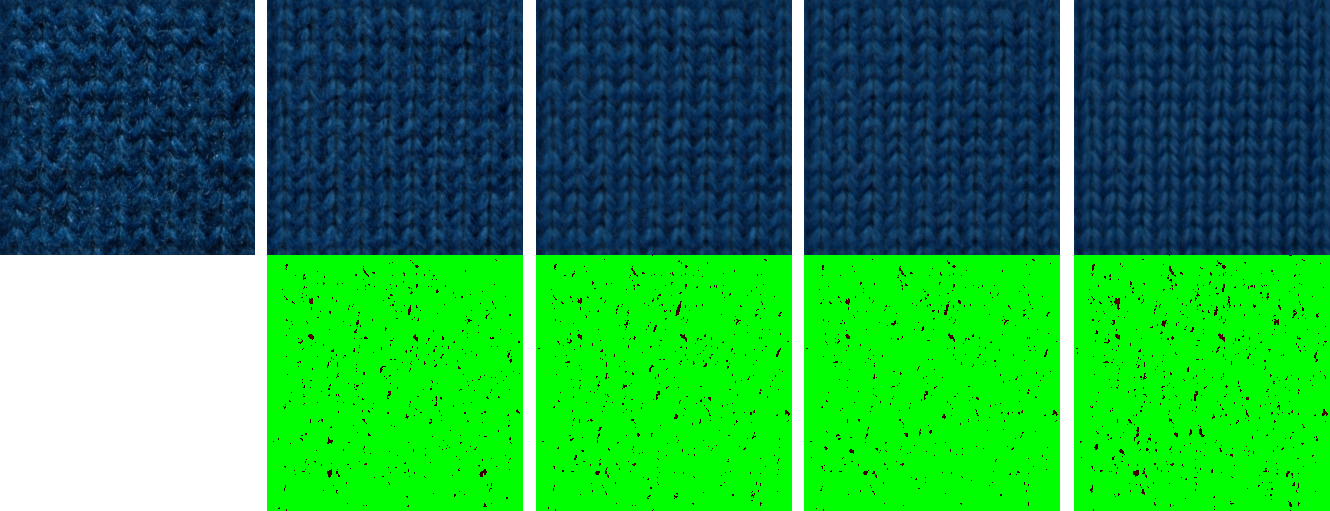
\includegraphics[width=1.0\textwidth]{figures/differ}
 \caption[Example of decompression errors ] {
 	{\bf Example of decompression errors }

	\textbf{First row} from the left to the right: original image, \textbf{32} components (MAE:2.17), \textbf{16} components (MAE:1.83), \textbf{8} components (MAE:2.21), \textbf{4} components (MAE:3.04). 
	\textbf{Second row}: the difference between the original and the decompressed images, \emph{red} color denotes how big the error, \emph{green} denotes that the error is absent or very small.}
 \label{fig:compression_example}
\end{figure}




 Figure \ref{fig:compression_example} shows that the decompression error is not improved enormously for $16$ or even for $32$ components.
 That is why the reasonable choice is $8$ components, while for $4$ components the image getting blurred. Also, Haindl claims that $8$ components is the optimal number of components for the PCA RF \cite{haindl}, which is close to our method.



 
\begin{table}[h]
\begin{tabular}{|l|l|l|c|c|c|c|c|}
\hline
     & k                      & C                      & \begin{tabular}[c]{@{}c@{}}MAE\\  CIELab\end{tabular} & \begin{tabular}[c]{@{}c@{}}MAE \\ RGB\end{tabular} & \begin{tabular}[c]{@{}c@{}}RMSE\\  RGB\end{tabular} & \multicolumn{1}{l|}{Compression Ratio} & \begin{tabular}[c]{@{}c@{}}Parameters Size /\\  Storage Size (PNGs)\end{tabular} \\ \hline
wool & \multicolumn{1}{c|}{1} & \multicolumn{1}{c|}{8} & 2.14                                                  & 5.86                                               & 7.5                                                 & 1:23                                   & 53Mb / 20 Mb                                                                     \\ \hline
wool & 3                      & \multicolumn{1}{c|}{8} & 2.19                                                  & 6.83                                               & 8.68                                                & 1:70                                   & 18Mb / 5Mb                                                                       \\ \hline
wool & 3                      & 32                     & 2.22                                                  & 5.92                                               & 7.5                                                 & 1:17                                   & 70Mb / 25Mb                                                                      \\ \hline
\end{tabular}
\caption{ Evaluation of BTFs}
\label{table:mytable}
\end{table}


 Table \ref{table:mytable} provides the evaluation for the whole BTF space of the wool sample, i.e. for all possible camera and light directions.
 MAE is also computed in RGB color space and in addition Root Mean Square Error
 
 {\centering $RMSE = \sqrt{\frac{1}{N}\sum_{i=1}^{N}(y_i-\hat{y_i} )^2}$\\}

 RMSE gives large weights to big errors, thus we can evaluate the variance of the errors \cite{rmse}.
 The bigger the RMSE the bigger the variance. We can see that in our case the RMSE is close to the MAE, which means that the variance of the errors is relatively small.
 
In the first row of the  Table \ref{table:mytable} where $k=1$ our method becomes equal to the PCA RF \cite{haindl} method.
Haindl claims to have the MAE equal to $3.16$ in CIELAB color space for the same sample \cite{haindl}.
 Our method produces a bit better result, i.e. $2.14$. 
 The second row shows that for  $k=3$ MAE stays practically the same. 
 However, the compression ratio improves in three times!
 We can see that even for $32$ components the decompression errors improves only a bit, but the compression ratio becomes worse.
 If we use $k$ bigger than $3$, then we would need to use more components to have good decompression error.
 For intance, our method becomes equal to PCA BTF \cite{haindl} when $k=81$ (all the camera directions). In this case we would need approximately $41$ components \cite{haindl}.
 Haindl has the MAE equal to 2.85 for the PCA BTF and compression ratio $1:23$ \cite{haindl}. 
 This means  $k=81$ and $C=41$ is not the optimal configuration too, because it would be computational heavy task for the GPU to do computation for $41$ components.
 
 Also, LPCA BTF \cite{haindl} has MAE equal to $2.42$, which is practically equal to our method. 
 However, we use $8$ components, while LPCA BTF uses $19$ on average.
 
 

\section{Real-time performance}
\label{section:eval_streaming}

We evaluate the rendering quality during the streaming and the real-time performance.
Our demo viewer is available at  http://btf.mywebcommunity.org. 
Figure \ref{fig:streamPreview} depicts the results of the evaluation.
We tested our approach on three materials: wool, impalla and corduroy.
The configuration of the compression is $k=3$ and $C=8$.

\begin{figure}[h]
 \centering
 \includegraphics[width=1.0\textwidth]{figures/streampreview}
 \caption[Example of Progressive Streaming ] {
 	{\bf Example of Progressive Streaming}

	\textbf{From left to right}: \emph{1}, \emph{2}, \emph{4}, \emph{6}, \emph{8}  components rendered at the same accordingly.
	}
 \label{fig:streamPreview}
\end{figure}
\label{chapter:implementation}

Rendering starts as soon as the first component transfers to the client side.
 The overall appearance of the the material is already visible even with the first the component, which has the size on average about $0.7$Mb.
With further components the overall quality of the image improves, i.e. specularities are increasing, small micro-structures become more visible and emphasized.
After all components are transmitted, the viewer hits the maximum available frame-rate on the average GPU.
The demo-viewer works well even on the mobile devices.

